\documentclass[12pt,a4paper]{amsart}
\usepackage[utf8]{inputenc}
\usepackage{amsmath}
\usepackage{amsfonts}
\usepackage{amssymb}

\usepackage{hyperref}

\usepackage{float}
\usepackage{subfig}


\usepackage{graphicx}
\usepackage{caption}
%\usepackage[nobysame, alphabetic]{amsrefs}
%\usepackage{here}
%\usepackage{showkeys}
\newcommand{\modif}{$\clubsuit$}
\newtheorem{thm}{Theorem}[section]
\newtheorem{defn}[thm]{Definition}
\newtheorem{coro}[thm]{Corollary}
\newtheorem{prop}[thm]{Proposition}
\newtheorem{lem}[thm]{Lemma}
%\theoremstyle{definition}
\newtheorem{rmk}[thm]{Remark}
\newtheorem{cond}[thm]{Condition}

%CB defs
\def\HH{\mathbb{H}}
\def\KK{G_4}
\def\dHH{\partial \mathbb{H}}
\def\HHn{\HH^n}
\def\hd{\hat{\delta}}
\def\ha{\hat{\alpha}}
\def\haa{\ha \cup \{\alpha^+,\alpha^-\}}

\def\im{\mathrm{Im}\,}
\def\SL{\mathrm{SL}(2,\CC)}
\def\xx{\HH/g2}


\def\ZZ{\mathbb{Z}}
\def\CC{\mathbb{C}}
\def\RR{\mathbb{R}}
\def\QQ{\mathbb{Q}}
\def\NN{\mathbb{N}}

\def\tt{\Sigma_{1,1}}

\def\fp{\mathbb{F}_p}
\def\aut{\text{Aut}(\F2)}
\def\gl2{\mathrm{GL}(2, \ZZ)}
\def\sl2{\mathrm{SL}(2, \ZZ)}
\def\g2{\Gamma(2)}
\def\slc{\mathrm{SL}(2, \CC)}

\def\xx{\HH/\g2}
\def\gg{X\cup X'}
\def\ggp{X}

\def\isom{\mathrm{isom}(\HH)}

\def\isomH{\text{isom}^+(\HH)}
\def\tr{\text{tr\,}}


\def\GI{\mathbb{Z}[i]}
\def\hc{\CC \setminus \GI}



\title{Geometry of Fermat's sum of squares}

 \author[McShane]{Greg McShane}
 \author[Vlad]{Vlad Sergiescu}
\address{Institut Fourier 100 rue des maths, BP 74, 38402 St Martin d'H\`eres cedex, France}
\email{mcshane at univ-grenoble-alpes.fr}


\begin{document}

\maketitle

\begin{abstract} 
We prove Fermat's sum  of two squares theorem 
using well known calculations from hyperbolic geometry 
and considerations of automorphisms of the three punctured sphere.
\end{abstract} 

\section{Introduction}


Consider the following pair of well known theorems from elementary number theory:

\begin{thm}\label{triv}
Let $p$ be a prime then the equation
$$x^2 = -1$$
admits a solution in $\fp$ iff 
$p=2$ or $p-1$ is a multiple of $4$.
\end{thm}


\begin{thm}[Fermat]\label{main}
Let $p$ be a prime then the equation
$$x^2 + y^2 = p $$
has a solution in integers  iff  $p=2$ or $p-1$ is a multiple of $4$.
\end{thm}

These results are intimately linked and often one deduces the second as a corollary of the first,
 for example, by using unique factorisation in the Gaussian integers.  We present a unified geometric  approach to these results  using the theory of group actions and in particular an application of Burnsides's lemma. 
 
 
As in Zagier's remarkable proof \cite{zagier} 
(see also \cite{heath,north,aigner2,elsholtz} for closely related constructions and discussion)
both results follow from showing that a certain involution has a fixed point. Amusingly Burnsides's lemma reduces this to showing that another involution has exactly two fixed points:
\begin{itemize}
\item  In the proof of Theorem \ref{triv} this is a consequence of the fact that a quadratic equation 
over a field has at most two solutions.
\item In the proof of Theorem \ref{main} this follows from some geometry and the fact that 
	every odd prime can be written in an essentially unique way
	as the difference of two squares $a^2 - b^2$.

% $$ \det 
% \begin{pmatrix}
% k + 1 & k- 1\\
% p & p 
% \end{pmatrix} = 2p \neq 2.
% $$

 \end{itemize}


\subsection{Organisation and Remarks}

In Section 2 we recall the statement of Burnside's lemma 
and apply it to a Klein four group generated by involutions of $\fp^*$
yielding a proof of Theorem \ref{triv}. In Section 3 we introduce $\g2$
and the associated Riemann surface $\xx$. 
In Section 4, for each prime $p$
we study how the automorphisms of $\xx$ 
act on a family of geodesic on this surface
obtained in a natural way from the rationals $k/p$.
In particular we show 
% (Lemma \ref{the end})  
that if $p$ is congruent to 1 modulo 4
there is always an orientation preserving involution that
leaves one of our geodesics invariant
and from this we deduce Theorem \ref{main}.

\subsubsection{Heath-Brown's proof}

In 1984 Heath-Brown published a proof of Theorem \ref{main}
apparently  in the journal of the Oxford University undergraduate mathematics society. 
His proof arose from a study of the account of Liouville’s papers on identities for parity functions, presented  by Uspensky and Heaslet in the 70s. Zagier's proof in \cite{zagier} is a clever reformulation of ths argument.

Like our  proof it is based on the action of a Klein four group on a
finite set and considerations of parity. To define his set
Heath-Brown introduces an auxiliary equation namely 

$$p = 4xy + z^2$$ 

whereas in our proof the sum of squares decomposition arises
directly as the  result of a geometric construction. As such, the
motivation for our work is to show that the finite sets involved in
the proof can be chosen to be both natural and have a geometric
interpretation. For example, in Section 2 we give a proof of Theorem
\ref{triv} using a group generated by 


$$ \begin{array}{lll} x
&\mapsto& -x \\ x &\mapsto& 1/x \end{array} $$

and in the proof of Theorem \ref{main} our group is generated by 

$$
\begin{array}{lll} z &\mapsto& -\bar{z} \\ z &\mapsto& 1/\bar{z}
\end{array}. $$



\subsubsection{Burnside's lemma and signatures}
 The astute reader will surely realise that Burnside's lemma is not essential to our argument
 and that one can achieve the same reduction by considering the signature
 of the permutations associated to the  involutions we consider. 
 This approach is closer to the parity arguments in Heath-Brown \cite{heath}.
% In fact the first author set this as an  undergraduate exam question some years ago.
 
 \subsubsection{Farey tessalation, $\lambda$-lengths}

 Much of our inspiration for this approach comes from  endless
 contemplation of the \textit{Farey tessalation}.
 
 The idea of associating a length to a geodesic joining cusps
 (paragraph \ref{lengths}) appears in Penner's work on moduli
 \cite{bob},
see also \cite{spring} for a more recent account.
He defined the $\lambda$-length of simple bicuspidal geodesic 
on a punctured
surface to be the exponential of half the 
length of the portion outside of some fixed
system of cusp regions.
Though not strictly necessary 
we will phrase parts of proof in terms of $\lambda$ lengths
as this is the origin of the  intuition behind our approach. 
Lemma \ref{calcul} shows that in the context we consider
a $\lambda$-length is always the determinant 
of an integer matrix.

In \cite{bob} Penner presents an approach to the Markoff equation
using $\lambda$-lengths. Alternatively,  using the existing calculations in
Wolpert \cite{saw} one can show that, for a suitable choice of cusp
region on the modular torus  the $\lambda$-lengths of arcs coincide
with the squares of Markoff numbers. Then, using the fact that each
arc is invariant under the elliptic involution one can show, using
Lemma \ref{squares}, that every Markoff number is the sum of two
squares. In fact this was the observation that was the starting
point for this paper.
% and we give a short exposition of it  in the appendix.
 
 
 \subsubsection{Bézouts Theorem}
 We are implicitly using  Bézout's Theorem
 (and in particular in the proof of Lemma \ref{action})
 when we assert that
 \begin{itemize}
 \item $\sl2$ is transitive on $\QQ \cup \infty$ (which is equivalent to Bézout's Theorem.)
 \item $\g2$ has exactly three orbits on $\QQ \cup \infty$.
 \end{itemize}
In fact Lemma \ref{action} can be proved
 without using our notion of length for a bicuspidal geodesics 
 but  instead by studying the action of 
 the lifts $U$, $V$  of the generators of our group $\KK$  
 and applying Bézout's Theorem.
 
 
 \subsubsection{References}
Almost all  of the material in Sections 3 and 4 
can be found in Serre's book \cite{serre} and the reader
should not need any other references to understand 
this paper if they are already familiar with  Burnside's lemma.
 

\subsection{Thanks}

The first author thanks Louis Funar and the second author for  many
useful conversations over the years concerning this subject. He would
also like to thank Xu Binbin for reading early drafts of the
manuscript.


\section{Burnside's Lemma} \label{burnside}

We give a proof of Theorem \ref{triv} using Burnside's Lemma.
Recall that if $G$ is  a group acting on a finite set $X$ then
Burnside's lemma says

\begin{equation}\label{class formula}
|G| |X/G| = \sum_{g} |X^g| 
\end{equation}  

where, as usual, 
 $X^g$ denotes the set of fixed points of the element $g$ 
 and $X/G$  the orbit space.


Let $p \neq 2$,  $X = \fp^*$ and $G$ be the group generated by the two involutions
\begin{eqnarray*}
x & \mapsto -x \\
x & \mapsto 1/x.
\end{eqnarray*}
The group  $G$ has exactly four elements namely:
\begin{itemize}
\item the trivial element which has  $p-1$ fixed points
\item $x\mapsto -x$ which has no fixed points 
\item  $x\mapsto 1/x$ has exactly two fixed points namely $1$ and $-1$.
\item  $g:x \mapsto -1/x$ is the remaining element and the theorem is equivalent to the existence of a fixed point for it.
\end{itemize}
Note that since $\fp$ is a field 
$|X^g| = \sharp \{x^2 = -1, \, x\in \fp^* \}$
is either $0$ or $2$.
Now for our choice of $X$ and $G$ equation (\ref{burnside}) yields
\begin{equation}
4 |X/G|   = (p-1) + 2 + |X^g|.
\end{equation}  
The LHS is always divisible by $4$ so the  RHS is too and
it follows from this that
$$ |X^g|. = \left\{  \begin{array}{ll}
0 & (p-1) =  2 \mod 4 \\
2 & (p-1) =  0 \mod 4 \\
\end{array}
\right.
$$
This proves Theorem \ref{triv}.

\subsection*{Note}
As was noted in the introduction one can obtain the same conclusion 
by calculating the signature of $x\mapsto -1/x$ 
using the fact that it is  the composition of
$x \mapsto -x$ and $x \mapsto 1/x$.


\section{Reciprocals of sums of squares and arcs}

This group of integer matrices $\sl2$  acts on $\HH$ by linear fractional transformations
that is:
$$\begin{pmatrix}
a & b \\
c & d
\end{pmatrix} \in \sl2,\, z\in \HH,\, 
\begin{pmatrix}
a & b \\
c & d
\end{pmatrix}. z = \frac{az + b}{cz + d}.
$$
The key lemma that relates this  $\sl2$ action to sums of squares is Lemma \ref{squares}.
\subsection{Ford circles, lengths, midpoints} 
\label{lengths}
Lemma \ref{squares} illustrates the connexion between sums of squares,
the orbit $\sl2.i$ and Poincaré geodesics. 
We now recall some standard ideas from hyperbolic geometry
which in particular will allow us to give an intuitive definition 
of our set $X$ in the next section.
We define an \textit{arc} to be a Poincaré geodesic
with endpoints in $\partial \mathbb{H}$ a pair of extended rationals, 
that is elements of $\mathbb{Q} \cup \infty$.

We denote by $F$ the set  $\{ z, \im z > 1\}$
this is a \textit{horoball in $\mathbb{H}$} centered at $\infty$.
The image of $F$ under the $\sl2$ action consists of
$F$ and infinitely many disjoint discs, 
which we will refer to as \textit{Ford circles}, 
each tangent to the real line at some rational $m/n$.
We adopt the convention that $F$ is also a Ford circle of infinite radius
tangent to the extended real line at $\infty = 1/0$.


\begin{figure}[ht]

	\begin{center} 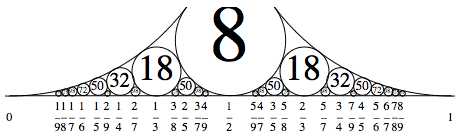
\includegraphics[scale=.8]{Ford-circles.png}
	\end{center}

\caption{Ford circles with tangent points and curvatures. Recall
that the curvature of a euclidean circle is the reciprocal of the
square of its radius.}%needs checking \end{figure}
\end{figure}


The following is well known and is easily checked:

\begin{lem}\label{ford}.

\begin{enumerate}
\item The Ford circle tangent to the real line at $m/n$
has Euclidean diameter $1/n^2$.

\item The closures of a  pair of distinct Ford circles are either disjoint or meet in a 
point of the $\sl2$-orbit of $i$.
\end{enumerate}
\end{lem}

%Two Ford circles are adjacent iff their closures meet in a point
%and this point is invariably a point of the orbits $\sl2.i$


Let $a/c, b/d$ be a pair of distinct rationals.
We define the \textit{length} of the arc 
joining these rationals 
%$\{ k/p + i t,\, t >0 \}$
%$F$ to the Ford circle tangent at $k/p$.
to be the length, with respect to the Poincar\'e metric on $\HH$, 
of the portion of this arc 
outside of the Ford circles tangent at $a/c, b/d$ .
Further we define its  \textit{mid point} to be the midpoint of this sub arc.
%We remark that if the projection of the line to $\xx$
%is invariant by an automorphism 
%then the midpoint is necessarily a fixed point of the automorphism.

\begin{figure}[ht]
\begin{center}
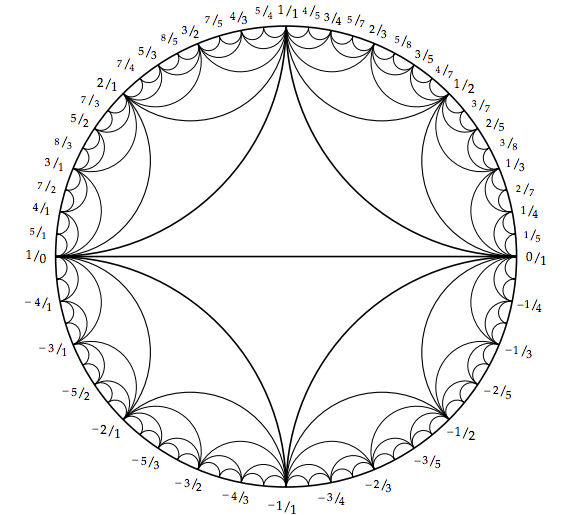
\includegraphics[scale=.5]{farey_diagram.png} 
\end{center}
\caption{Farey diagram.}
\label{farey diagram}
\end{figure}


Following Penner \cite{bob}, 
see also \cite{spring} for a more recent account,
we define the
$\lambda$-length of the arc to be the exponential of half
of this length.

\begin{lem}\label{calcul}
Let $a/c, b/d$ be a pair of distinct extended rationals.
Then the  $\lambda$-length of the arc joining them
 is the absolute value of the determinant of the matrix
$$\begin{pmatrix}
a & b \\ c & d
\end{pmatrix}.$$

Further if $a/b = 1/0$ then the arc is a vertical line 
 whose midpoint has imaginary part equal to $1/d$ .
\end{lem}

\proof
By transitivity of the $\sl2$ action on the extended rationals
we may suppose $a/b = 1/0 = \infty$.
The arc joining $a/c, b/d$ is a vertical line and 
the determinant of the matrix in the statement  is just $d$.
By Lemma \ref{ford} the Ford circle tangent at $b/d$ 
has diameter $1/d^2$ so the portion of the arc 
outside $F$ (the Ford circle tangent at $\infty$) 
and this circle is a segment between $z_1$ with imaginary part 1
and $z_2$ with imaginary part $1/d^2$.
A standard calculation using the Poincaré metric $\frac{dz}{\mathrm{Im} z}$
shows that the length of this segment is indeed $\log (d^2)$. 
The second part of the statement follows from a similar calculation.
\hfill $\Box$.

The arcs of $\lambda$-length 1 are the edges in the so-called 
\textit{Farey diagram} (see Figure \ref{farey diagram}).

\subsection{Sums of squares}

\begin{lem} \label{squares}
Let $n$ be a positive integer.
The number of  ways of writing $n$  as a  sum of squares
$$n = c^2 + d^2$$
with $c,d$ coprime positive  integers
is equal to the number of  integers $0 \leq k < n-1$ coprime to $n$
such that the line
$$\{  k/n + i t,\, t >0 \}$$
contains  a point in the $\sl2$  orbit of $i$.
\end{lem}


\proof  Suppose there is such  a point which we denote  $w$.
The point $w$ is a fixed point of some  element of order 2 in $\sl2$.
Since the Ford circles are $\sl2$ invariant
this element must permute $F$ with the Ford circle tangent 
to the real line  at the real part of $w$.
So, in particular, $w$ is the midpoint of the line 
that it lies on 
and by  Lemma \ref{calcul} one has:

$$\frac{1}{n} = \im \frac{1 }{n}(k + i)  
= \im  \frac{ai +b}{ci+d }
= \frac{\im i} {c^2 + d^2}.$$

Conversely if $c,d$ are coprime integers 
 then there exists $a,b$ such that
 $$ad - bc = 1 \Rightarrow  
 \begin{pmatrix}
 a & b \\
 c & d
 \end{pmatrix} \in \sl2.
$$
%The real part of $w = \frac{ai +b}{ci+d }$ is
%$$ac + bd = (a,b).(c,d),$$
%and
By applying a suitable iterate of the parabolic transformation 
$z \mapsto z + 1$,
one can choose $w$ such that $0 \leq \text{Re\,} w < 1$.
So if $n = c^2 + d^2$ then $\frac{ai +b}{ci+d }$
is on one of the lines of the family in the statement.

\hfill $\Box$


\subsection{Relation with square roots of $-1$}

Suppose that $p$ is a prime as in Section \ref{burnside}.
In fact the real part of 
$\frac{ai +b}{ci+d }$ is related to the square
root of $-1$ in $\fp$ in a simple way:
begin by writing
$$
 \frac{ai +b}{ci+d }
= \frac{m}{p} + \frac{i}{p}
$$
then 
$$
\frac{m^2 + 1}{p^2}   
% = \left (\frac{m}{p} + \frac{i}{p}\right)
% \overline{\left (\frac{m}{p} + \frac{i}{p}\right)}
= \left( \frac{ai +b}{ci+d }\right) 
\overline{\left( \frac{ai +b}{ci+d }\right)}
= \frac{a^2 +b^2}{c^2+d^2 }
$$
 now since $p = c^2 + d^2$ one has:
 \begin{eqnarray}
 m^2 + 1
=  p(a^2 + b^2).
\end{eqnarray}
Thus $m$ determines a square root of $-1$ in $\fp$. 

\section{The three punctured sphere}

In this section we are concerned with the geometry of the surface
$\xx$ associated to $\g2$, the principal level 2 congruence subgroup
of $\sl2$. This group acts on $\ZZ^2$, that is pairs of integers,
preserving parity.

 \begin{figure}[hb]
\begin{center}
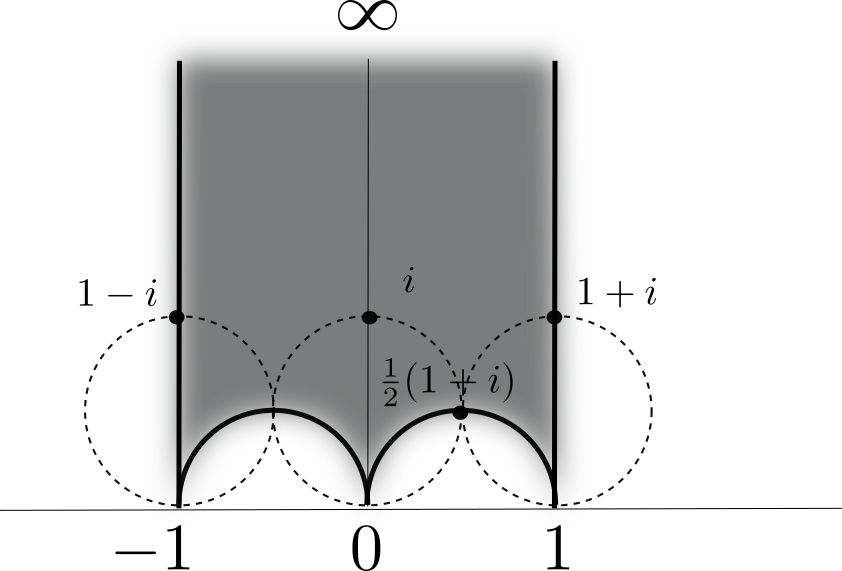
\includegraphics[scale=.5]{fund_dom.png} 
\end{center}
\caption{Standard fundamental domain for $\g2$ and its decomposition into ideal triangles.}
\label{fund}
\end{figure}


It also acts on $\HH$ by linear fractional transformations that is:

$$\begin{pmatrix}
a & b \\
c & d
\end{pmatrix} \in \sl2,\, z\in \HH,\, 
\begin{pmatrix}
a & b \\
c & d
\end{pmatrix}. z = \frac{az + b}{cz + d}.
$$

The quotient $\xx$ is conformally equivalent to the Riemann  sphere
minus three points which we will refer to as \textit{cusps} (see
Figure \ref{3punctured}). Following  convention we label these cusps
$0,1,\infty$ respectively, corresponding to the three $\g2$ orbits
of $\QQ \cup \infty$. Finally, the \textit{standard fundamental
domain}  for $\g2$ is the convex hull of the points $\infty, -1, 0 ,
1$. This region can be decomposed into two ideal triangles $\infty,
-1, 0 $ and $ 0 , 1,\infty$ as in Figure \ref{fund}. The edges of
the ideal triangles project to three disjoint simple geodesics on
$\xx$ and each edge has a \textit{midpoint} which is a point of the
$\sl2$ orbit of $i$ (see Figure \ref{3punctured}).




 \begin{figure}[hb]
\begin{center}
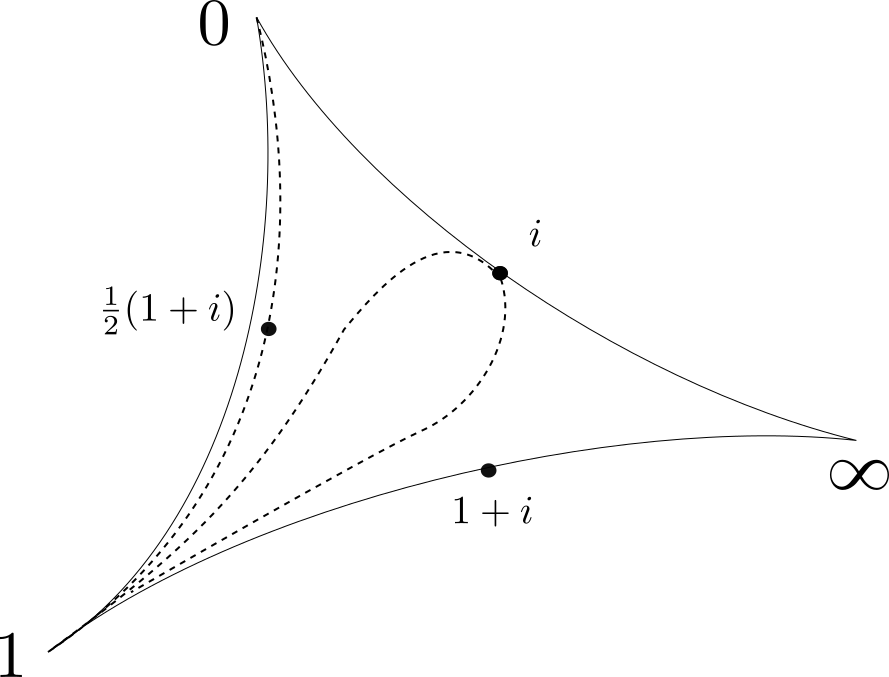
\includegraphics[scale=.5]{3sphere.png} 
\end{center}
\caption{Three punctured sphere with cusps and midpoints labelled.
The dotted loop is the fixed point set of the automorphism induced by $V'$.}
 \label{3punctured}
\end{figure}





\subsubsection{Cusp regions}

The image of a Ford circle on $\xx$ is a \textit{cusp region}
around one of the three cusps $0,1,\infty$.
Pairs of these cusp regions are tangent at one of the midpoints
labelled $i, 1+i, \frac12(1+i)$.
It is not difficult to see that these cusp regions 
are permuted by the automorphisms of $\xx$.
It follows that if an automorphism preserves a geodesic  joining cusps on $\xx$
then it must permute the Ford regions at each end of a lift to $\HH$.


\subsection{Automorphism groups of $\xx$}
From covering theory an isometry  of $\HH$ 
induces an automorphism of $\xx$ iff it normalises the covering group
i.e. $\g2$.
It follows that,
since $\g2$ is a normal subgroup of $\sl2$,
 the quotient group
$$H^+: = \sl2/\g2$$
acts as a group of (orientation preserving) automorphisms of the surface $\xx$.
More generally, $\g2$ is normal in $\gl2$ and 
$$H: = \gl2/\g2$$
acts as a group of possibly orientation reversing  automorphisms of the surface $\xx$.


\subsection{Orientation reversing automorphisms}
To prove Theorem \ref{main} we will have to work with automorphisms
that do not preserve the orientation and in particular 
those induced by the involutions:
\begin{eqnarray*}
U: z &\mapsto& -\bar{z} \\
V: z &\mapsto& 1/\bar{z} 
\end{eqnarray*}
Both $U$ and $V$ normalise $\g2$ so induce automorphisms of $\xx$. Note
that
the composition of $U$ and $V$ is none other than the involution
$$ z \mapsto -1/z,$$
so we have a Klein 4-group as in Section \ref{burnside}.


\begin{lem}
The group $\KK$ descends to a group of automorphisms 
on the three punctured sphere which preserve the cusp labelled $1$ (see Figure \ref{3punctured}).
\end{lem}

\proof

One checks that each of the generators $U$ and $V$ preserve the
standard fundamental domain and further they preserve the set
$\{1,-1\}$. Note that this pair of points belong to the same $\g2$
orbit and so project to the same cusp on $\xx$. It follows that the
generators preserve this cusp ie the cusp labelled $1$.

\hfill $\Box$
% Strictly speaking, for the proof of Theorem \ref{main} this lemma is irrelevant 
% as all we require is that the group contains a suitable Klein four group.


\subsection{Fixed point sets }

Recall that  $\KK$,  the group generated by $U,V$,
Consider the fixed point sets of the elements:
\begin{itemize}
\item $U$ fixes the  vertical line $\{ it, t >0 \} $;
\item $V$ fixes the  semi circle  joining $-1$ and $1$;
\item $U\circ V(z) = -1/z$  and so fixes $i$.
\end{itemize}
From this we may deduce that the automorphisms of $\xx$ induced by $U$ and $V$ 
each fix a pair of lines on the surface. 
The fixed point set of  $V$ projects 
to a geodesic on $\xx$ (depicted as a dotted loop in Figure \ref{3punctured})
separating the surface
 into  two pieces which are permuted by 
the corresponding automorphism,
so the fixed point set is exactly this geodesic.
For $U$ the fixed point set of the induced automorphism  is strictly bigger 
as it will also fix  the images on the surface of 
$\{1+  it, t \in \RR \} $ 
and the semi circle joining $0$ to $1$.
This is because
these arcs are sides of the standard fundamental domain for $\g2$:
\begin{itemize}
	\item
$U(1+  it) = - 1+  it = f(1+  it),$
where $ z \mapsto z - 2$ is the side-pairing for these sides.
	\item
$U$ exchanges 
the semi circle joining $0$ to $1$
and the semi circle joining $0$ to $-1$
and these sides are paired by $z \mapsto z/(2z +1)$ 
\end{itemize}

This proves the first part of:

\begin{lem} \label{the fixed point}
	
	Any arc of the Farey diagram projects to a component of the
	fixed point set of the automorphism induced by $U$ ob $\xx$.

	The fixed point set of the automorphism induced by $U\circ
	V$  is exactly the intersection of the fixed point sets of
	the automorphisms induced by $U$ and $V$. This is  a single
	point namely the image of $i$ on $\xx$

\end{lem}

\proof 

% % The standard  fundamental domain for the action of $\g2$ 
% % is the convex hull of $\infty, -1, 0 , 1$.
% % This can be decomposed into two ideal triangles (as in Figure \ref{fund})
% % with vertices $\infty, -1, 0 $ and $ 0 , 1,\infty$ respectively.
% The fixed point set $\gamma$ of $U$
% is an arc in the Farey diagram which 
% is invariant under $\g2$
% so any lift of the induced automorphism
% is also an arc of the Farey diagram.
% One checks that the projection of any arc of the Farey diagram is fixed by the automorphism induced by $U$.


The second part of lemma follows from the observation that 
$U\circ V$ leaves the standard fundamental domain for $\g2$
invariant swapping the two ideal triangles in the complement
of the the fixed point set of $U$.
One sees from this that any fixed point
of $U\circ V$ is contained in the fixed point set of $V$.
Further, $U\circ V$ fixes the cusp labeled $1$
but exchanges the cusps labeled $0$ and $1$.
It follow that any fixed point of $U \circ V$
is contained in the projection of the vertical 
line $\{ it, t >0 \}$.
This line contains $i$ and the lemma is proven.

\hfill $\Box$

\section{Action on a family of arcs}

Now $\KK$ permutes the cusps labelled $\infty$ and $0$  on $\xx$
and will obviously permute the geodesics joining them.
If $\gamma$ is such a geodesic then
any  lift
$\hat{\gamma} \subset \HH$ is an arc joining a point in the 
$\g2$ orbit of $\infty$ to another in the  $\g2$ orbit of $0$
and so $\gamma$ has a well defined $\lambda$ length.
For any integer $n$ $\KK$  permutes the set of geodesics joining the 
cusps labelled $\infty$ and $0$  on $\xx$
of $\lambda$-length $n^2$.
This will be our set $X$.


\subsection{Canonical lifts}

Let $n$ be an integer and 
$N'$  the set of integers coprime with $n$.
Consider the collection of geodesics of $\HH$.
$$\{  k/n+ i t,\, t>0  \},\, k \in N'.$$
The image of this collection on the quotient surface $\xx$ a family of arcs
% of $2\phi(n)$ 
and, since $\Gamma(2)$ preserves parity, these split into two sub families namely:
\begin{itemize}
\item those joining the cusps labelled $\infty$ and $0$ that is belonging our set $X$
\item those joining the cusps labelled $\infty$ and $1$.
\end{itemize}
The first of these sub families consists of projections of the lines
$$\hat{X} :=  \{  2k/n+ i t,\, t >0 \},\, k \in N'$$


\begin{lem} \label{action}
Let $p$ be a prime then the set $X$ consists of $p-1$ elements.
\end{lem}
\proof
The $z \mapsto z + 2$ is a generator of the subgroup of $\g2$ that stabilises $\infty$ so to have a complete set of representatives of $\hat{X}$ we need only consider $2k/n$ with $0 < k < n$. If $n$ is prime then for any such $k$ $2k$ and $n$ are coprime so $\hat{X}$ contains exactly $n-1$ elements.

\hfill $\Box$


 
 \section{Proof of Fermat's Theorem}

Throughout this section the integer $n$ is a prime which we denote $p$.
Theorem \ref{main} follows from:

\begin{lem} \label{midpoint}
Let $p$ be a prime congruent to 1 or 2 modulo 4.
Then there is always a geodesic 
in the family $\hat{X}$
that has as its  midpoint a point in the $\sl2$  orbit of $i$.
\end{lem}

This is equivalent to saying that, on projecting to the surface
$\xx$, there  is always a geodesic in $X$ which passes through the
fixed point of the map induced by $U \circ V$. For $p=2$ this can be
done explicitly and for the general case by the argument using 
Burnside's lemma in Section \ref{burnside} it suffices to show that:

\begin{itemize}
	\item $U$ fixes no element of $X$
	\item $V$ fixes at most two.
\end{itemize}

\subsection{The singular case of Lemma \ref{midpoint}}

The case $p=2$ is exceptional and we will deal with it first.
From the preceding paragraph there is a single geodesic namely 
the projection of the line 
$$\{ 1/2 + i t,\, t \in \RR \}$$
and this contains the point  $\frac{1}{2 }(1+ i)$
Note that one has 
$$\begin{pmatrix}
1 & 0 \\
1 & 1
\end{pmatrix} \in \sl2,\,\, \begin{pmatrix}
1 & 0 \\
1 & 1
\end{pmatrix}.i  = \frac{1}{2 }(1+ i)$$
so this point is in the $\sl2$ orbit of $i$>
Then one has as in Lemma \ref{squares}:
$$\im \frac{1}{2 }(1+ i) = \frac{1}{2}  =  \im \begin{pmatrix}
1 & 0 \\
1 & 1
\end{pmatrix}.i = \frac{\im i}{ 1^2 + 1^2}$$
So, in a rather roundabout way, we obtain $2$ as a sum of squares by comparing denominators:
$$2 = 1^2 + 1^2.$$


\subsection{Inversions and fixed points in $X$}

We will finish the proof of  Lemma \ref{midpoint}
by showing that there is a geodesic invariant by 
the orientation preserving automorphism in $\KK$,
obtaining the required midpoint as the fixed point of the automorphism induced by $U\circ V$.
Our  argument is exactly  the same as for
 Theorem \ref{triv}.
 More precisely, we show that, for any  $p > 2$:
\begin{enumerate}
\item the automorphism induced by $U$ preserves no geodesic in  $\ggp$
\item the automorphism induced by $V$ preserves at most two geodesics in $\ggp$
\end{enumerate}

%\subsubsection{Conjugations between  inversions}
The first point is rather easy 
(the automorphism induced by $U$ fixes three disjoint geodesics joining 
cusps and permutes the pair of ideal triangles in their complement)
 but the second requires establishing
 the analogue of the fact that  the equation
$$x^2 = 1$$
has at most two solutions in any field or integral domain for that matter. 

Let us start by 
considering the action of $V$
on the set of rationals, recall that
$$V: z \mapsto 1/\bar{z}$$
so that for coprime integers $a,b$
$$a/b \mapsto b/a.$$
If $a/b \neq \pm 1$ 
then this map preserves the
geodesic joining $a/b$ and $b/a$
and the $\lambda$-length of this arc is
$$|a^2 - b^2|.$$
So if this is to be a lift of one of our arcs
$$ a^2 - b^2 = \pm p$$
and since $p$ is prime the only solutions
must satisfy (after possibly permuting $a,b$):
$$a + b = \pm p,\, a - b = \pm 1.$$
Thus up to changing sign
$$a = \pm(p + 1)/2,\,  b = (p-1)/2.$$
Thus we have:

\begin{lem}\label{just two}
The automorphism induced by $V$ preserves two and exactly two geodesics in $\ggp$.
\end{lem}


\subsection{Composite integers}

It is well known that the set of integers $n$ 
which can be written as a sum of squares 
$c^2 + d^2$ with $c,d$ coprime is (almost) closed under
multiplication:
if $p,q$ are sums of squares and at least one is odd then the
product is also a sum of squares. 
For example one has
$$50 = 5^2 \times 2 = | (1+2i)^2 (1+i) |^2 = |  -7 + i |^2 = 7^2 + 1^2 $$
and
$$65 = 5 \times 13 = | (1+2i)(2+3 i) |^2 = |  -4 + 7i |^2 = 7^2 + 4^2.$$
but of course 
$$ 20 = 2 \times 10= |(1 + i)(1+ 3i)|^2 = | -2 + 4i |^2 = 2^2 + 4^2.$$

Despite this multiplication by $2$ seems to have a nice geometric interpretation
in the spirit of our analysis of arcs but multiplication by $5$
does not seem to have one.
Let $p$ be a prime such that $p-1$ is a multiple of $4$
and $m$ a square root of $-1$ then 
$\frac{m}{p} + \frac{i}{p}$
is a point of the $\g2$-orbit of $i$.
The semi circle joining $\frac{m-1}{p}$ to  $\frac{m+1}{p}$
has $\lambda$-length $2p$
and passes through 
$\frac{m}{p} + \frac{i}{p}$.
So by Lemma \ref{squares} $2p$ is a sum of squares.

It seems difficult to prove that $65$ is a sum of squares directly
using our approach with Burnside's lemma and considering  the set
$X$ of arcs of $\lambda$-length $65$. Naively applying Burnside's
lemma yields:

$$4 |X/G|   = \phi(65)+  |\{ x, x^2 = 1 \}| + |\{ x, x^2 = -1 \}| = 48 + 4 +  |\{ x, x^2 = -1 \}|.$$

\subsubsection{The Ptolemy Identity and multiplicativity}


Looking at this equation modulo 4 is not helpful. However, by using
the fact that $\lambda$-lengths satisfy the Ptolemy Identity one can
prove a weaker form of the closure property quite easily.

\begin{figure}[ht]
\begin{center}
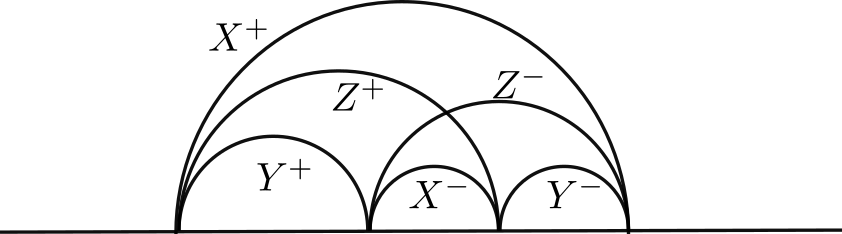
\includegraphics[scale=.5]{ptolemy.png} 
\end{center}
\caption{Ptolemy Identity diagram.}
\label{Ptolemy}
\end{figure}

The \textit{Ptolemy Identity} concerns the $\lambda$-lengths of an
ideal quadrilateral see Figure \ref{Ptolemy}. If $X^\pm, Y^\pm$ are
the  $\lambda$-lengths of pairs of  opposite sides and $Z^\pm$ of
the diagonals then

\begin{equation}
	X^+ X^-
	+ Y^+ Y^- = Z^+ Z^-
\end{equation}

Now suppose that $p,q$ are distinct integers which can be written as
sums of squares, by Lemma \ref{squares} there is a pair of arcs on
$\xx$ with $\lambda$-lengths $p$ and $q$ respectively which meet in
the projection of $i$ to the surface. In the upper half space $\HH$
there is a corresponding pair of lifts that intersect in $i$. The
convex hull of these arcs is an ideal quadrilateral in $\HH$ to
which we can apply the Ptolemy Identity. Observe that in addition
this quadrilateral is invariant under $z \mapsto -1/z$ so $X^+ =
X^-$ and $Y^+ = Y^-$, such a quadrilateral is a
\textit{parallelogram} for $\lambda$-length, and we have

\begin{equation}
	(X^+)^2 + (Y^+)^2 = pq.
\end{equation}

\begin{figure}[ht]
\begin{center}
	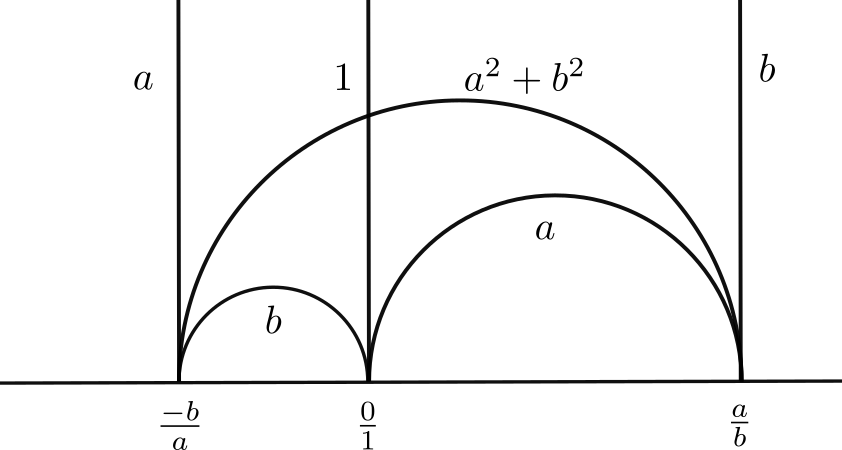
\includegraphics[scale=.5]{./p2_quad.svg.png}
\end{center}
\caption{A $\lambda$-length parallelogram 
invariant under $z\mapsto -1/z$. Its vertices are $\infty, -b/a, 0,
a/b$. This illustrates a special case of the Ptolemy Identity.}
\label{pythagoras}
\end{figure}

Note that if $p,q$ are square free and coprime then $X^+$ and
$Y^+$ are automatically coprime though this may not be the case in
general so more work is required to prove the strong form of closure
under multiplication.

If $q=p>2$ then find an arc in $\HH$ passing through $i$ and of
$\lambda$-length $p$. The image of the arc under $z \mapsto \bar{z}$
also passes through $i$ and has $\lambda$-length $p$. Now proceed as
before to obtain an ideal parallelogram
which represents $p^2$ as a sum of squares.
Note that this fails for $2$ as the initial arc joins $-1$ to $1$
and so is invariant under $z \mapsto \bar{z}$.

\section{Concluding remarks}

We have given a geometric treatment of Fermat's theorem
using the automorphisms of the surface
$\xx$ and Penner's $\lambda$-lengths. In another work we will study
the relation between the quadratic form $x^2 +xy + y^2$ and $\xx$.

%\begin{LARGE}
%
%
%CAN YOU SEE WHY VLAD ?
%
%\end{LARGE}


% \section{Appendix: Markoff numbers}

% We discuss the connection between $\lambda$-lengths
% and Markoff numbers showing that every such number is 
% the sum of two squares without applying Theorem \ref{main}.
% We then proceed to show uniqueness for Markoff numbers
% satisfying certain arithmetic conditions (Theorem \ref{button})
%  following Baragar and Button
%  see also \cite{mong,zhang,zhang2} for alternative approaches.
% The content of this appendix is purely expository and,
% as such,
% we make no claims of originality.
% We will assume that the reader has some familiarity with 
% the theory of Fuchsian groups.


% \begin{thm}
% For each  Markoff triple $(X,Y,Z)$
% there is a (unique) ideal triangulation of the modular torus
% such that the $\lambda$-lengths of the arcs are 
% $X^2,Y^2,Z^2$.
% \end{thm}

% \subsection{Markoff cubic}

% A \textit{Markoff triple} is a  solution $(X,Y,Z)$  in positive integers to
% the \textit{Markoff cubic}
% \begin{equation}\label{m cubic}
% X^2 + Y^2 + Z^2 - 3XYZ = 0.
% \end{equation}
% A \textit{Markoff number} is an integer in a Markoff triple.
% H. Cohn showed that Markoff numbers are related to the 
% lengths of simple closed geodesics on the \textit{modular torus}
% that is $\HH/\Gamma'$ 
% where $\Gamma' < P\sl2$ is the commutator subgroup.
% More precisely, if $\gamma$ is such a geodesic then :
% \begin{equation}
% X  = \frac{2}{3} \cosh \left( \frac{\ell_\gamma}{2}\right),
% \end{equation}
% is a Markoff number where $\ell_\gamma$ is the length of $\gamma$.
% Conversely, every Markoff number arises from a geodesic length.

% \subsection{Character Variety}

% It is convenient to change variables and study solutions off
% \begin{equation}\label{f cubic}
% X^2 + Y^2 + Z^2 - XYZ = 0.
% \end{equation}
% By the work of Fricke the set of solutions in positive real numbers
% can be identified with a certain slice of the 
% \textit{relative character variety of $\ZZ * \ZZ$}.
% This is the set of  representations 
% $$\rho: \ZZ * \ZZ \rightarrow SL(2, \RR)$$
% such that the trace of the image of the commutator of the generators is $-2$
% up to conjugation.
% The key point in Fricke's work is that an (irreducible) representation $\rho$
% is determined up to conjugation by the three numbers
% \begin{eqnarray*}
% X &= &tr \rho(\alpha), \\
% Y  &= &tr \rho(\beta), \\
% Z &= & tr \rho(\alpha\beta)),
% \end{eqnarray*}
% where $\alpha,\beta$ are generators of $\ZZ*\ZZ$.
% Fricke calculates the trace of the commutator and shows that
% \begin{equation}
% 2 + tr\,  (\alpha\beta\alpha^{-1}\beta^{-1}) = X^2 + Y^2 + Z^2 - XYZ .
% \end{equation}
% The quotient surface $\HH/\rho(\ZZ*\ZZ)$ is invariably a once punctured torus
% and we identify $\ZZ * \ZZ$ with its fundamental group.
% The $\alpha\beta\alpha^{-1}\beta^{-1}$ is a loop around the puncture
% and the condition of the trace means that the monodromy around this loop is parabolic.


% \subsection{$\lambda$ lengths}

% There is an embedded cusp region $H$ of area $2$ 
% on the punctured torus $\HH/\rho(\ZZ*\ZZ)$
% (see \cite{thesis} for a discussion).
% By replacing $\rho$ by a conjugate representation
% we may assume $\rho(\ZZ*\ZZ)$  that 
% $$\rho(\alpha\beta\alpha^{-1}\beta^{-1}): z \mapsto z + 6,$$
% it follows that $H$ lifts to the set $\hat{H} = \{ \im z > 3 \}$.
% Let $\alpha*$ be an\textit{arc} that is a bicuspidal geodesic
% without self intersetions.
% There is a lift of $\alpha*$ to $\HH$ which is a vertical line
% which evidently meets $\hat{H}$,
% we claim that any lift of of $\alpha*$ 
% which meets $\hat{H}$ is a vertical line and not a semi circle.
% For, if $C$ is a semi circle that meets $\hat{H}$ 
% its diameter is strictly greater than $6$ 
% and it follows that $C$ and $C + 6$ meet transversely in some point$x$.
% Such a point gives rise to a self intersection on the quotient surface
% It follows that, the portion of $\alpha^*$ outside of $H$ is connected,
% and define and we define  $\lambda$ length 
% to be the exponential of the length of this sub arc.

% \begin{lem}\label{lambda length}
% Let $\alpha*$ be an arc on a once punctured torus 
% and $\alpha$ the unique 
% simple closed geodesic disjoint it.
% Then the square root of the $\lambda$-length  of the arc $\alpha$
% is equal to $\frac{2}{3}\cosh \ell_\alpha / 2$.
% \end{lem}

% It is possible to prove this directly using hyperbolic trigonometry 
% following the same schema as in \cite{thesis}
% but here we give a more conceptual proof  using the computations from \cite{saw}.

% Given an arc $\alpha^*$ one may extend it to an ideal triangulation off the punctured torus:
% that is there is a pair of arcs $\beta^*,\gamma^*$, each disjoint from  $\alpha^*$ and their complement 
% is a pair of ideal tirangles. 
% Let $X$ denote $2 \cosh \ell_\alpha / 2$ where $\alpha$ is the unique closed simple 
% geodesic disjoint from $\alpha$.
% \begin{eqnarray*}
% Y &=& 2 \cosh \ell_\beta / 2 \\
% Z  &=& 2 \cosh \ell_\gamma / 2 \\
% \end{eqnarray*}
% where $\beta$ resp $\gamma$ is the unique closed simple  geodesic disjoint from
% $\beta^*$ resp. $\gamma^*$.

%   \begin{figure}[ht]
% \begin{center}
% 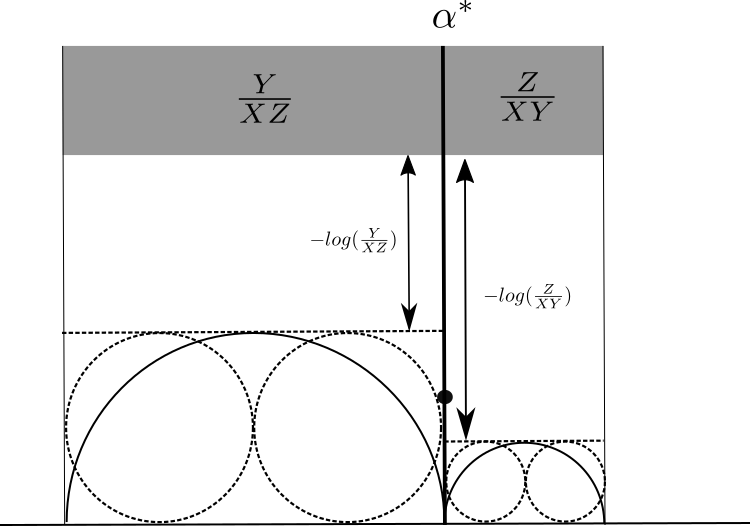
\includegraphics[scale=.5]{shear.png} 
% \end{center}
% \caption{Calculating the hyperbolic length of $\alpha^*$ in the upper half plane
% the $\lambda$-length is the exponential of this.
% The mid point of $\alpha^*$ is marked by a circle and
% the two corners adjacent to $\alpha^*$ are shaded}
% \label{penner}
% \end{figure}

% In  \cite{saw} Wolpert divides the Markoff cubic by $XYZ$ to obtain
% $$\frac{X}{YZ} + \frac{Y}{XZ} + \frac{Y}{XZ} = 1.$$
% The three terms in this relation have a geometric interpretation
% which we will exploit to compute the $\lambda$-length of $\alpha^*$.
% Let $H$ denote the cusp region of area $2$. 
% A\textit{corner} of an ideal triangle is one of the 
% three components of its intersection with $H$.
% Every torus admits an \textit{elliptic involution}
% which leaves each of the arcs of the ideal triangulation  invariant
%  and swaps the triangles.
% So, in fact, to each triangulation we can associate three numbers
% namely the areas of the corners of one of the  ideal triangles
% and these coincide with Wolpert's three numbers.

% Lifting the ideal triangulation to $\HH$ as in Figure \ref{penner}
% one sees that  $\alpha^*$ decomposes into two arcs of length
% $-\log(Y/XZ)$ and $-\log(Z/XY)$ respectively
% so that its is of length $2\log X$.

% So, on any hyperbolic punctured torus,
% the $\lambda$-length of $\alpha^*$ wrt the cusp region of area 2 is
% the exponential of this, that is:
% $$ X^2.$$
% Now on the modulaire torus $\HH/\Gamma'$ there is an embedded cusp 
% region of area 6 and the $\lambda$-length of $\alpha^*$ wrt this cusp region
% is
% $$ \frac{X^2}{9}.$$



% \subsection{Sum of squares}\label{frobenius}


% In the proof of Lemma \ref{lambda length} 
% we used the fact that
% every torus admits an \textit{elliptic involution}
% which leaves each of the arcs of the ideal triangulation  invariant
%  and swaps the triangles.
% For the modular torus the involution is covered by $z \mapsto -1/z$ 
% and  this means that for any arc $\alpha^*$ every lift contains a point 
% of the $\sl2$-orbit of $i$.
%  In particular, by Lemma \ref{lambda length},
%  a lift which is a vertical line ends at a rational 
%  which has as denominator a Markoff number
%  and so this Markoff number is a sum of two squares.
%  Conversely, every Markoff number arises as the square of a $\lambda$-length
%  of some arc  $\alpha^*$ and so must be the sum of two squares.
%  By extending this reasoning slightly one may show:
 
%  \begin{thm}
% Frobenius' conjecture is equivalent to:
% Let $m$ be a Markoff number then exactly one of the vertical lines
% with endpoint  $k/m$, where $1\leq k \leq m-1$ is coprime to $m$,
% projects to an arc on the modular torus.
% \end{thm}

% \proof The Markoff triples form a binary tree with a preferred vertex corresponding to
% the fundamental triple $(1,1,1)$. 
% Define the multiplicity of a Markoff number to be the  number of triples for which
% it appears as the largest integer.
% One can easily check that for the so-called singular Markoff numbers 1 and 2
% their multiplicity is 3
% and, since,
% group of automorphisms of the tree that fix the fundamental triple of order 6
% that the multiplicity of any other Markoff number is at least $6$.
% Thus Frobenius' conjecture can be restated as:
% multiplicity of any other Markoff number is at most $6$.

% Using Cohn's correspondence it follows that Frobenius' conjecture
% is equivalent to: 
% the number of oriented closed simple geodesics on the modular torus
% of any given length is at most 6.
% Each (unoriented) closed simple geodesic is disjoint from exactly one arc
% so that there can be at most three arcs of any given $\lambda$-length.

% The group of orientation preserving  automorphisms of the modular torus 
% is canonically isomorphic to 
% $$\sl2 / \Gamma' \simeq \ZZ/3\ZZ \times \ZZ/2\ ZZ \simeq \ZZ/6\ZZ .$$
% The commutator of the generators of $ \Gamma'$  is $z \mapsto z + 6$
% and since each automorphism $\phi$ must leave the cusp invariant it lifts to
% a map of the form $\hat{\phi} : z \mapsto z + k,\, k= 0,\dots 5$.
% Now consider the lift of some arc on the modular torus 
% which, WLOG, is a vertical line. 
% After applying (the lift of)  an automorphism $\hat{\phi}$ 
% we may assume it has its end point in $\RR$ between $0$ and $1$.
% The statement now follows by counting multiplicities as before.

% \hfill $\Box$
 
%  \subsection{Uniqueness of Markoff Numbers}
 
%  Frobenius' conjecture says that the largest number in a Markoff triple determines
%  the remaining two numbers \cite{aigner}. Button and Baragar (see chapter 10 of Aigner \cite{aigner})
%  used  basic algebraic algebraic number to show that certain Markoff numbers satisfied
%  the uniqueness conjecture. Subsequently Aigner extended used this approach showing:
 
%  \begin{thm}[Aigner]
%  Let $m$ be a Markoff number of the form 
%  $$m =Np^k$$
%  where $p$ is an odd prime and $N \leq 10^{35}$ is another Markoff number. Then $m$ is unique.
%  \end{thm}
 
%  This is a strengthening a result from Button's thesis:
 
%   \begin{thm}[Baragar, Button, Schmutz] \label{button}
%  Let $m$ be a Markoff number of the form 
%  $m=p^k$ or $m=2p^k$ then it is unique
% if $p$ is an odd prime.
%  \end{thm}

% We give a short proof of this using the fact that the Gaussian integers
%  is a unique factorisation domain.

% \proof: Suppose that $m=p^k$ is a Markoff number. By the previous paragraph there are coprime integers $a,b$ so that 
% $$p^k = a^2 + b^2 \Rightarrow a^2b^{-2} = -1 \in \fp.$$
% It follows that $p$ is either $2$ or $1 \mod 4$ and 
% so by Theorem \ref{main} there are coprime positive integers $c,d$,
%  unique up to permutation,
% so that  $$p = c^2 + d^2 = (c + id)(c - id).$$
% It is well known that the RHS is the unique factorisation of $p$ in the Gaussian integers
% and it follows that the unique factorisation of $m$ is
% $$p^k = (c + id)^k(c - id)^k.$$
% A consequence of this is that the pair coprime positive integers $a,b$ such that $p^k = a^2 + b^2$
% is unique up to permutation. Explicitly we have:
% \begin{eqnarray}
% a &=& \mathrm{Re}\, (c\pm id)^k \\
% b &=& \mathrm{Im}\, (c\pm id)^k.
% \end{eqnarray}
% Since $a,b$ are unique up to permutation 
% then, by Lemma \ref{squares},
%  there can only be a single  geodesic of the family
% of vertical lines ending at  
% $k/p^k$ which meets the $\sl2$-orbit of $i$.
% The result follows immediately from the  Paragraph \ref{frobenius}.

% Now suppose that  $m=2p^k$ is a Markoff number.
% By the above  $p^k$ can be written as a sum of squares $a^2 + b^2 = |a + ib|^2$ 
% essentially uniquely.
% Observe that   $2$ factors as 
% $$ 2 = i(1+i)^2.$$
% Observe that $2 p^k$ can also  be written as a sum of squares
% essentially uniquely namely
% $$2p^k = |(1+i) (a + ib) |^2 =  (a-b)^2 + (a+b)^2,$$ 
% so that the result follows in this case too.



% \hfill $\Box$


%Finally we show that a result of Zhang \ref{zhang2} 
%can be treated in exactly the same manner:
%
%  \begin{thm}
% Let $m$ be a Markoff number such that $3m -2$
% is either a prime power or twice a prime power
% then $m$ is unique.
% \end{thm}
% 
% \proof Consider the Markoff cubic
% $$X^2 + Y^2 + Z^2 - 3XYZ = 0.$$
% If we consider it as a quadratic in $Z$ we see that it has two solutions $Z^\pm$
% which satisfy (one of) the Vieta relations 
% $$ Z^+ + Z^- = 3XY.$$
% So that if $Z^-$ is a Markoff number then $Z^+ = 3XY- Z^-$ is also.

 
 


 
 


%
%  \begin{figure}[ht]
%\begin{center}
%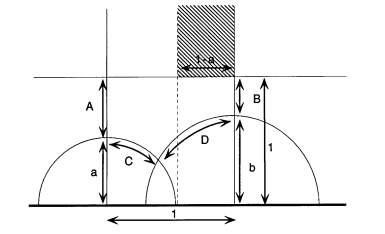
\includegraphics[scale=1]{lifts.png} 
%\end{center}
%\caption{Lifting to $\HH$. 
%The capital letters are hyperbolic lengths
%whereas small letters are Euclidean lengths.
%Note that the two semi circles meet perpendicularly
%and in particular $a^2 + b^2 = 1$}
%\label{arcs}
%\end{figure}
%
%\proof
%The proof is contained in  Figure \ref{arcs} (Fig. 5 from \cite{thesis}).
%The horizontal line represents the boundary 
%of the cusp region of area $4$ and not $2$.
%We can still use the diagram to calculate the $\lambda$-length:
%we must multiply by a factor of $4$ to get the correct result.
%
%\begin{itemize}
%\item 
%$B$ is the half the length of the portion
% arc $\alpha*$ outside the cusp region 
%An elementary calculation shows that  $B = -\log b$
%and so the $\lambda$-length of $\alpha*$ is $4/b^2$.
%\item 
%$C$ is half the length of the closed geodesic  $\alpha$
%and from an elementary calculation yields 
%$$C= \log (1/b+ a/b) = \log ((1+a)/b).$$
%\end{itemize}
%So since $a^2 + b^2 = 1$ one has:
%$$ 2 \cosh C = \frac{1+a}{b}  + \frac{b}{1+a } = \frac{1 + 2a + (a^2 + b^2)}{(1+a)b} = 
% \frac{2}{b}.$$
%
%Thus the $\lambda$-length is $4/b^2$
% 
%\hfill $\Box$
%



%\subsection{Ideal triangulations}
%

%
%



\thebibliography{99}

% \bibitem{aigner}
% M. Aigner
% \textit{Markov's Theorem and 100 Years of the Uniqueness Conjecture}, Springer( 2013)

\bibitem{aigner2}
Aigner M., Ziegler G.M.  
\textit{Representing numbers as sums of two squares.} In: Proofs from THE BOOK. Springer, Berlin, Heidelberg. (2010)

% \bibitem{barag}
% A. Baragar,
% \textit{On the Unicity Conjecture for Markoff Numbers}
% Canadian Mathematical Bulletin , Volume 39 , Issue 1 , 01 March 1996 , pp. 3 - 9

% \bibitem{button}
% J. O. Button, 
% \textit{The uniqueness of the prime Markoff numbers},
%  J. London Math. Soc.
% (2) 58 (1998), 9–17.

% \bibitem{cana}
% Ilke Canakci, Ralf Schiffler
% \textit{Snake graphs and continued fractions}
% European Journal of Combinatorics
% Volume 86, May 2020, 103081

\bibitem{elsholtz}
Elsholtz C.A 
\textit{Combinatorial Approach to Sums of Two Squares and Related Problems.}
 In: Chudnovsky D., Chudnovsky G. (eds) Additive Number Theory. Springer, New York, NY.
 (2010) 

\bibitem{felikson}
\textit{Ptolemy Relation and Friends,}
Anna Felikson,
preprint arXiv:2302.06379

\bibitem{ford}
Lester R Ford,
\textit{Automorphic Functions}

\bibitem{heath}
Heath-Brown, Roger. 
\textit{ Fermat’s two squares theorem.} Invariant (1984) 

% \bibitem{thesis}
% G. McShane,
% \textit{Simple geodesics and a series constant over Teichmuller space}
% Invent. Math. (1998)

% \bibitem{mong}
% M.L. Lang, S.P Tan,
% \textit{A simple proof of the Markoff conjecture for prime powers}
% Geometriae Dedicata volume 129, pages15–22 (2007)

\bibitem{bob}
R. C. Penner, 
\textit{The decorated Teichmueller space of punctured surfaces}, 
Communications in Mathematical Physics 113 (1987), 299–339.


\bibitem{north}
Northshield, Sam. 
\textit{A Short Proof of Fermat’s Two-square Theorem.} The American Mathematical Monthly. 127. 638-638. (2020). 

\bibitem{serre}
J-P. Serre,
\textit{A Course in Arithmetic},
Graduate Texts in Mathematics,
Springer-Verlag New York
1973

\bibitem{spring}
B. Springborn. The hyperbolic geometry of Markov's theorem on
Diophantine approximation and quadratic forms. Enseign. Math.,
63(3-4):333--373, 2017. doi:10.4171/LEM/63-3/4-5.

\bibitem{saw}
Scott Wolpert,
\textit{On the Kahler form of the moduli space of once-punctured tori}, 
Comment. Math. Helv. 58(1983)246-256

\bibitem{zagier}
D. Zagier,
 \textit{A one-sentence proof that every prime p = 1 (mod 4) is a sum of two squares}, 
 American Mathematical Monthly, 97 (2): 144
 
 % \bibitem{zhang}
 % Y. Zhang,
 % \textit{ An elementary proof of uniqueness of Markoff numbers}
 % preprint, arXiv:math.NT/0606283
 
  % \bibitem{zhang2}
  %  Y. Zhang,
 % \textit{Congruence and uniqueness of certain Markoff numbers}
 % Acta Arithmetica, Volume: 128, Issue: 3, page 295-301




%\bibitem{mcp}
%Greg McShane, Hugo Parlier,
%Multiplicities of simple closed geodesics and hypersurfaces in Teichmüller space,
%Geom. Topol.
%Volume 12, Number 4 (2008), 1883-1919.
%
%\bibitem{mcr}
%Greg McShane, Igor Rivin
%\textit{A norm on homology of surfaces and counting simple geodesics}
%International Mathematics Research Notices, Volume 1995, Issue 2, 1995
%
%
%
%\bibitem{ra}
%M. Rabideaua, R. Schiffler,
%\textit{Continued fractions and orderings on the Markov numbers},
%Advances in Mathematics Vol 370,  2020.
%
%
%
%\bibitem{vu}
%C Lagisquet and E. Pelantová and S. Tavenas and L. Vuillon,
%\textit{On the Markov numbers: fixed numerator, denominator, and sum conjectures.}
%\url{https://arxiv.org/abs/2010.10335}
%


%\bibitem{Gui}
%L. Guillop\'e, Laurent(F-GREN-F)
%Sur la distribution des longueurs des g\'eod\'esiques ferm\'ees d'une surface compacte \`a bord totalement g\'eod\'esique. 
%Duke Math. J. 53 (1986), no. 3, 827-848. 

%\bibitem{MC}
%C. L. Mallows and J. M. C. Clark. 
%{\it Linear-intercept distributions do not characterize plane sets}
% Journal of Applied Probability, 7(1):240-244, 1970.
% 
% \bibitem{Masai-McShane}
% Masai, Hidetoshi and Greg McShane,
% ``On systoles and ortho spectrum rigidity'', preprint.
% \bibitem{MMc}
% Masai, Hidetoshi, and Greg McShane. "Equidecomposability, volume formulae and ortho spectra." Algebraic \& Geometric Topology 13.6 (2013): 3135-3152.
 



\end{document}


For the pair $\infty, 1/2$  and  $0, 2/p$   one has the matrix equation:
\begin{equation}
\begin{pmatrix}
1 & 1\\
0 & 2
\end{pmatrix}
= 
\begin{pmatrix}
 -(p-1)/2& 1\\
1 & 0
\end{pmatrix}
\begin{pmatrix}
0& 2\\
1 & p
\end{pmatrix}.
\end{equation}


The first matrix on the LHS is an element of $\gl2$
and from it, using Lemma \ref{fps}, we can obtain an orientation reversing isometry of
$\HH$ conjugating the inversion (\ref{inversion}) to $V$.
Finally, by changing signs in the expression(\ref{inversion})  one obtains an inversion 
conjugate to $V$ mapping the geodesic with endpoint $-1/p$ to itself.

%We say that a pair of (extended) rational $m/n, m'/n'$ are \textit{Farey neighbors} 
%if $|mn' - nm'| = 1$ with the convention that $\infty = 1/0$ 
%so that it's neighbors are exactly the integers $m/1$.
%The Farey neighbors of $0= 0/1$ are the rationals $1/n$ and in particular $1/p$ 
%is one of them though $2/p$ is not. 
